\documentclass[border=3pt]{standalone}
% Preâmbulo compartilhado pelos diagramas TikZ da aula 7 (Filtros Não Paramétricos)
\usepackage[T1]{fontenc}
\usepackage[utf8]{inputenc}
\usepackage{lmodern}
\usepackage{amsmath}
\usepackage{xcolor}
\usepackage{tikz}
\usetikzlibrary{arrows.meta,angles,quotes,decorations.pathmorphing,calc,
                positioning,shapes.geometric,shapes.misc,backgrounds,fit,
                math}

% Paleta (mesma dos SVGs originais)
\definecolor{dblue}{HTML}{2A5B8C}
\definecolor{dorange}{HTML}{B3541E}
\definecolor{dgreen}{HTML}{4A7C59}
\definecolor{dred}{HTML}{9C4B4B}
\definecolor{dcream}{HTML}{F4F1EA}
\definecolor{dshade}{HTML}{DDD7C9}

% Função gaussiana (não normalizada por padrão de escala visual)
\pgfmathdeclarefunction{gauss}{3}{%
  \pgfmathparse{1/(#3*sqrt(2*pi))*exp(-((#1-#2)^2)/(2*#3^2))}%
}

% Estilos comuns (prefixo d... para não colidir com chaves internas do pgf)
\tikzset{
  >={Stealth[length=2mm]},
  dguide/.style={gray!55, dashed, line width=0.4pt},
  daxis/.style={gray!60, line width=0.7pt, ->},
  dbody/.style={fill=black!3, draw=black!80, line width=1pt},
  dacc/.style={draw=dblue, line width=1pt},
  dlbl/.style={black!55, font=\small},
  dsub/.style={black!45, font=\footnotesize},
  dstate/.style={circle, draw=black!80, fill=dcream, line width=1pt,
                 minimum size=17mm, font=\large, inner sep=1pt},
  dobs/.style={circle, draw=black!80, fill=dshade, line width=1pt,
               minimum size=14mm, font=\large, inner sep=1pt},
  dbox/.style={rounded corners=2pt, draw=black!80, fill=dcream, line width=1pt,
               align=center, inner sep=6pt},
  dop/.style={circle, draw=black!80, fill=white, line width=1pt,
              minimum size=6mm, inner sep=0pt, font=\small},
  dtrans/.style={->, dblue, line width=1pt},
  dmeas/.style={->, dorange, line width=1pt},
  dcurve/.style={line width=1pt, dblue},
  dcurveb/.style={line width=1.4pt, dorange},
}

\begin{document}
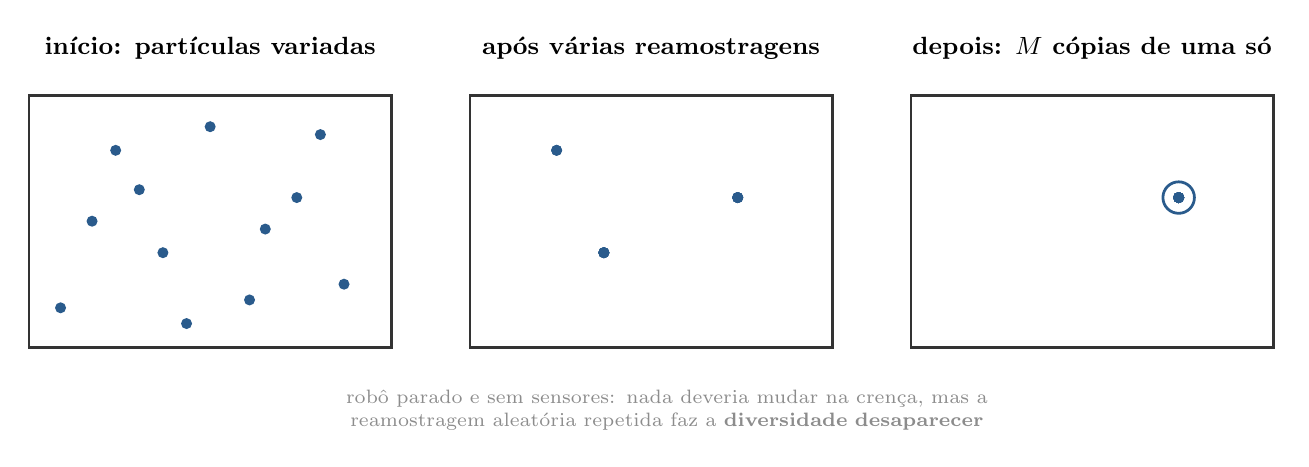
\begin{tikzpicture}[x=1cm,y=1cm]
  \newcommand{\planta}{\draw[dbody, fill=white, line width=1pt] (0,0) rectangle (4.6,3.2);}
  \begin{scope}
    \planta \foreach \x/\y in {0.4/0.5,1.1/2.5,1.7/1.2,2.3/2.8,2.8/0.6,3.4/1.9,4.0/0.8,0.8/1.6,3.7/2.7,2.0/0.3,1.4/2.0,3.0/1.5} { \fill[dblue] (\x,\y) circle (0.07); }
    \node[font=\small\bfseries] at (2.3,3.8) {início: partículas variadas};
  \end{scope}
  \begin{scope}[shift={(5.6,0)}]
    \planta \foreach \x/\y in {1.7/1.2,1.7/1.2,1.7/1.2,3.4/1.9,3.4/1.9,3.4/1.9,3.4/1.9,1.1/2.5,1.1/2.5,1.7/1.2,3.4/1.9,1.7/1.2} { \fill[dblue] (\x,\y) circle (0.07); }
    \node[font=\small\bfseries] at (2.3,3.8) {após várias reamostragens};
  \end{scope}
  \begin{scope}[shift={(11.2,0)}]
    \planta \foreach \k in {1,...,12} { \fill[dblue] (3.4,1.9) circle (0.07); }
    \draw[dblue, line width=1pt] (3.4,1.9) circle (0.2);
    \node[font=\small\bfseries] at (2.3,3.8) {depois: $M$ cópias de uma só};
  \end{scope}
  \node[dsub, font=\scriptsize, align=center, text width=15cm] at (8.1,-0.8) {robô parado e sem sensores: nada deveria mudar na crença, mas a reamostragem aleatória repetida faz a \textbf{diversidade desaparecer}};
\end{tikzpicture}
\end{document}
